% Options for packages loaded elsewhere
\PassOptionsToPackage{unicode}{hyperref}
\PassOptionsToPackage{hyphens}{url}
%
\documentclass[
  11pt,
]{article}
\usepackage{amsmath,amssymb}
\usepackage{lmodern}
\usepackage{iftex}
\ifPDFTeX
  \usepackage[T1]{fontenc}
  \usepackage[utf8]{inputenc}
  \usepackage{textcomp} % provide euro and other symbols
\else % if luatex or xetex
  \usepackage{unicode-math}
  \defaultfontfeatures{Scale=MatchLowercase}
  \defaultfontfeatures[\rmfamily]{Ligatures=TeX,Scale=1}
\fi
% Use upquote if available, for straight quotes in verbatim environments
\IfFileExists{upquote.sty}{\usepackage{upquote}}{}
\IfFileExists{microtype.sty}{% use microtype if available
  \usepackage[]{microtype}
  \UseMicrotypeSet[protrusion]{basicmath} % disable protrusion for tt fonts
}{}
\usepackage{xcolor}
\usepackage[margin=1in]{geometry}
\usepackage{graphicx}
\makeatletter
\def\maxwidth{\ifdim\Gin@nat@width>\linewidth\linewidth\else\Gin@nat@width\fi}
\def\maxheight{\ifdim\Gin@nat@height>\textheight\textheight\else\Gin@nat@height\fi}
\makeatother
% Scale images if necessary, so that they will not overflow the page
% margins by default, and it is still possible to overwrite the defaults
% using explicit options in \includegraphics[width, height, ...]{}
\setkeys{Gin}{width=\maxwidth,height=\maxheight,keepaspectratio}
% Set default figure placement to htbp
\makeatletter
\def\fps@figure{htbp}
\makeatother
\setlength{\emergencystretch}{3em} % prevent overfull lines
\providecommand{\tightlist}{%
  \setlength{\itemsep}{0pt}\setlength{\parskip}{0pt}}
\setcounter{secnumdepth}{5}
\newlength{\cslhangindent}
\setlength{\cslhangindent}{1.5em}
\newlength{\csllabelwidth}
\setlength{\csllabelwidth}{3em}
\newlength{\cslentryspacingunit} % times entry-spacing
\setlength{\cslentryspacingunit}{\parskip}
\newenvironment{CSLReferences}[2] % #1 hanging-ident, #2 entry spacing
 {% don't indent paragraphs
  \setlength{\parindent}{0pt}
  % turn on hanging indent if param 1 is 1
  \ifodd #1
  \let\oldpar\par
  \def\par{\hangindent=\cslhangindent\oldpar}
  \fi
  % set entry spacing
  \setlength{\parskip}{#2\cslentryspacingunit}
 }%
 {}
\usepackage{calc}
\newcommand{\CSLBlock}[1]{#1\hfill\break}
\newcommand{\CSLLeftMargin}[1]{\parbox[t]{\csllabelwidth}{#1}}
\newcommand{\CSLRightInline}[1]{\parbox[t]{\linewidth - \csllabelwidth}{#1}\break}
\newcommand{\CSLIndent}[1]{\hspace{\cslhangindent}#1}
\usepackage{dcolumn}
\usepackage{float}
\floatplacement{figure}{ht}
\usepackage{setspace}
\usepackage{fancyhdr}
\pagestyle{fancy}
\usepackage{lastpage}
\setlength{\headheight}{14.49998pt}
\addtolength{\topmargin}{-2.49998pt}
\usepackage{rotating, graphicx}
\renewcommand{\topfraction}{.85}
\renewcommand{\bottomfraction}{.7}
\renewcommand{\textfraction}{.15}
\renewcommand{\floatpagefraction}{.66}
\setcounter{topnumber}{3}
\setcounter{bottomnumber}{3}
\setcounter{totalnumber}{4}
\usepackage[hang,flushmargin]{footmisc}
\usepackage{lipsum}
\usepackage{etoolbox}
\usepackage{mlmodern}
\usepackage[T1]{fontenc}
\usepackage{enumitem}
\setlist{noitemsep}
\AtBeginEnvironment{quote}{\singlespace\vspace{-\topsep}\small}
\AtEndEnvironment{quote}{\vspace{-\topsep}\endsinglespace}
\providecommand{\keywords}[1]{\textbf{Keywords:} #1}

\usepackage{booktabs}
\usepackage{longtable}
\usepackage{array}
\usepackage{multirow}
\usepackage{wrapfig}
\usepackage{float}
\usepackage{colortbl}
\usepackage{pdflscape}
\usepackage{tabu}
\usepackage{threeparttable}
\usepackage{threeparttablex}
\usepackage[normalem]{ulem}
\usepackage{makecell}
\usepackage{xcolor}
\ifLuaTeX
  \usepackage{selnolig}  % disable illegal ligatures
\fi
\IfFileExists{bookmark.sty}{\usepackage{bookmark}}{\usepackage{hyperref}}
\IfFileExists{xurl.sty}{\usepackage{xurl}}{} % add URL line breaks if available
\urlstyle{same} % disable monospaced font for URLs
\hypersetup{
  hidelinks,
  pdfcreator={LaTeX via pandoc}}

\title{The Myth of the Myth of Independence:\\
A Critique of Binder and Spindel's Appraisal of the Fed}
\author{Zachary Thomas McDowell\\
BA \& MA in Political Science}
\date{\textbf{Updated}: August 02, 2022}

\begin{document}
\maketitle
\begin{abstract}
\singlespace The response to Desmond King's review of \emph{The Myth of
Independence} by one of the book's authors reveals one of two possible
critical flaws in their thesis that the relationship between Congress
and the Federal Reserve is best described as one of interdependence.
Binder fails to adequately address the most important of King's
critiques. This article expands on the points raised by King in a more
comprehensive manner than a book review allows for, with a particular
emphasis on contributing novel empirical analyses that cast further
doubt on the arguments positied by Binder.
\end{abstract}

\keywords{Inequality, Federal Reserve, Monetary Politics, Financial Crisis}

\let\thefootnote\relax\footnotetext{\lipsum[1][1-7]}

\thispagestyle{empty}

\newpage
\fancypagestyle{TOC}{%
    \fancyhead[R]{}
    \fancyhead[L]{}
}

\thispagestyle{TOC}
\tableofcontents
\listoffigures
\listoftables
\clearpage
\newpage

\fancypagestyle{INTRODUCTION}{%
    \fancyhead[R]{}
    \fancyhead[L]{}
}

\thispagestyle{INTRODUCTION}
\clearpage

\spacing{1.5}

\hypertarget{introduction}{%
\section*{Introduction}\label{introduction}}
\addcontentsline{toc}{section}{Introduction}

The politics of monetary policy is not the most popular subfield in
political science. Therefore, it was curious to see that in 2018, the
journal \emph{Perspectives on Politics} published an interesting
back-and-forth between two opposing sets of monetary politics scholars.
Sarah Binder and Mark Spindel are the authors of \emph{The Myth of
Independence}, which argues that the Federal Reserve has an
``interdependent relationship'' with Congress. Both institutions rely on
each other for different things, so neither is wholly dependent on nor
independent from the other, hence why Binder and Spindel refer to their
relationship as interdependent. On the other hand, Desmond King and
Lawrence Jacobs argue in their book, \emph{Fed Power}, that the Federal
Reserve is effectively independent of Congress and holds more
institutional power than it has at any point in its history. They argue
that the Fed's policies, under normal economic conditions, serve to
worsen economic inequality by favoring financial capital over
working-class Americans. The \emph{Perspectives on Politics} article is
unique in that it is structured as follows:

\begin{enumerate}
\def\labelenumi{\arabic{enumi}.}
\tightlist
\item
  King reviews \emph{The Myth of Independence}
\item
  Binder and Spindel respond to King's review
\item
  Binder and Spindel reviews \emph{Fed Power}
\item
  King and Lawrence respond to Binder and Spindel's review
\end{enumerate}

In their response, King and Lawrence summarize their main disagreements
with \emph{The Myth of Independence}, stating that ``Sarah Binder and
Mark Spindel view the Fed's actions as part of a dance with Congress
that is largely silent about the winners and losers outside of
Washington. By contrast, \emph{Fed Power} puts the distributional
consequences of the central bank's policy front and center, along with
the politics that produces them''
(\protect\hyperlink{ref-binder2018c}{Binder et al. 2018}, pg. 783). In
other words, King criticizes Binder and Spindel for not paying enough
attention to the distributional consequences concerning income and
wealth that result from Fed policies, nor do they appear to recognize
the actual amount of power held by the Fed.

It is notable that these respective teams of Fed scholars would come to
such diametrically opposed positions when it comes to the true nature of
the relationship between Congress and the Fed. On its face, the question
of whether or not the Fed is dependent on Congress would seem rather
straightforward. In reality, as all four scholars point out, the
quasi-governmental status of the Fed makes it difficult to study, given
that its semi-private status prevents much information from being public
accessible. But with that being said, there is enough public information
available to where one might reasonably expect professional academics to
be able to come to an agreement on a simple question like: What's the
relationship between Congress and the Fed?

\hypertarget{initial-issues}{%
\section{Initial Issues}\label{initial-issues}}

Moreover, King and Lawrence, in their joint response, list their top
four criticisms of \emph{The Myth of Independence}, wherein they posit
that Binder and Spindel:

\begin{enumerate}
\def\labelenumi{\arabic{enumi}.}
\tightlist
\item
  Overstate the Fed's ``deference to Congress and underappreciates the
  Fed's will and capacity to evade legislative control''
  (\protect\hyperlink{ref-binder2018c}{Binder et al. 2018}, pg. 783).
\item
  Underappreciate that the Fed ``is independent of the congressional
  budget appropriations process''
  (\protect\hyperlink{ref-binder2018c}{Binder et al. 2018}, pg. 783).
\item
  Omit any discussion of the phenomenon known as ``financialization''
  (\protect\hyperlink{ref-binder2018c}{Binder et al. 2018}, pg. 783).
\item
  Fail to recognize the clear institutional bias towards the wealthy,
  which can be seen in how ``the Fed's selective benefits for finance and
  the conduct of monetary policy produce clear winners among the most
  affluent'' (\protect\hyperlink{ref-binder2018c}{Binder et al. 2018},
  pg. 783).
\end{enumerate}

What bothers me, as a scholar, is how Binder and Spindel egregiously
failed to refute King and Lawrence on the actual terms he presented,
almost as if they were intentionally ignoring the crux of King's
criticisms because they had no way to counter him directly, instead
relying on obfuscation to defend their claims. Binder and Spindel
responded in such a way as to make it seem that they were avoiding the
critiques raised in a seemingly condescending way.

Before we can begin arguing about whether or not the Fed is dependent on
Congress, we must first define what we mean by ``dependent.'' Further,
we must also pin down the contextual and effective meaning of
``accountability'' when discussing the relationship between the two
institutions. In my view, passing legislation is but one part of the
matrix of components that constitutes what is necessary, but not
sufficient, to hold the Fed accountable. I'm more interested in
investigating whether or not it can be reasonably argued that the Fed,
by virtue of its dependency on Congress, has been \emph{meaningfully}
held accountable by Congress for its various failings.

Without descending into a pedantic discussion of how to best understand
and define accountability in its totality, my argument relies on the
incorporation of one critical element involved in an entity being held
accountable: for something to be held accountable, there must be at
least some longevity in the newly applied constraints. In the context of
the Fed, this would mean that any reforms passed by Congress would
effectively constrain a particular set of dissatisfying actions taken by
the Fed for the indefinite future, up to and until Congress legally
undoes such reforms.

\hypertarget{stasis-issues}{%
\section{Stasis Issues}\label{stasis-issues}}

The authors in question are not addressing each other, thus creating
stasis issues in this ``critical dialogue.'' It is frustrating to watch
accomplished and no doubt knowledgeable Fed scholars talk past each
other, but here we are. What follows is a systematic breakdown of the
myriad stasis issues I identified in my reading of the critical
back-and-forths presented in Binder et al.
(\protect\hyperlink{ref-binder2018c}{2018}).

\hypertarget{inequality-the-fed}{%
\subsection{Inequality \& the Fed}\label{inequality-the-fed}}

The most egregious example of Binder and Spindel missing the point is
how they respond to King's assertion that the Fed's post-2008 policy led
to higher levels of income inequality. To highlight the degree to which
they miss King's point, here are their respective words:

\begin{quote}
\textbf{King}: Undeniably, the Fed's interventions after the 2008 Great
Recession to prevent a collapse of the financial system in the United
States and globally spared many from job loss and misery\ldots{} it is
important to avoid a false equivalency between the gains for finance and
those for the general public. The Fed's policies delivered lopsided and
often concealed benefits for finance, the top 1\%, and the institutional
interests of the Federal Reserve Bank that enjoys more power and
autonomy than at any time in its 100-year history
(\protect\hyperlink{ref-binder2018c}{Binder et al. 2018}, pg. 780).
\end{quote}

\begin{quote}
\textbf{Binder \& Spindel}: Congress authorizes the Fed to make
emergency loans to banks---not to steer aid directly to homeowners. In a
crisis, monetary policy can affect the real economy by pumping credit
through the clogged plumbing of the financial system. And evidence from
progressive economists suggests that the Fed's unconventional bond
purchases reduced mortgage rates, making working- and middle-class
Americans better-off (\protect\hyperlink{ref-binder2018c}{Binder et al.
2018}, pg. 781).
\end{quote}

I've done my best to fairly and accurately represent each author's views
while being concise. If anyone has issues with how I've represented the
above exchange, I welcome any criticisms, given the subjective nature of
how I chose to shorten the respective quotes. That said, insofar as the
above quotes \emph{do} accurately and fairly represent the authors'
respective views concerning the Fed's role in contributing to the 2008
financial crisis and the subsequent worsening of income and wealth
inequality, on top of the aforementioned job losses and misery, Binder's
response is lacking, to say the least.

Pointing to the fact that Fed's bond buying supposedly ``reduced
mortgage rates, making working- and middle-class Americans better-off''
is tantamount to lauding an engineer for filling a single crack on a
fully broken dam. Binder's response implicitly under-emphasizes the
apocalyptic experiences felt by millions of Americans and citizens
worldwide. Thomas Piketty is arguably the premier scholar when it comes
to income and wealth inequality. In his book, \emph{Capital in the
Twenty-First Century}, Piketty argues two main, overarching points.
First, the fundamental contradiction of capitalism is that, many times
throughout the 18th to 21st centuries, the rate of return on capital
assets was greater than the rate of economic growth, which he
illustrates with the following simple expression: \emph{r}
\textgreater{} \emph{g}.
(\protect\hyperlink{ref-albertus2016a}{\textbf{albertus2016a?}}) argues
that, while Piketty's explanation is mostly accurate, the U-shaped
pattern of inequality ``only really holds for a handful of
industrialized economies and a subset of developing countries'' (pg.
49). Instead, the authors argue that the observed pattern of global
income and wealth inequality seen in the 20th century resulted from the
``political regime types and the social groups they empower, rather than
war and globalization''
(\protect\hyperlink{ref-albertus2016a}{\textbf{albertus2016a?}}, pg.
49).

There may not be enough time in this article to discuss the Fed's role
in propping up the European Union during the Eurocrisis, but it's at
least worth mentioning for the time being. For now, it is necessary to
specify what we mean when discussing and subsequently operationalizing
``economic inequality.''

The most common way scholars measure \emph{income} inequality is by
calculating a country's Gini coefficient, an index value ranging from 0
to 1, with 0 representing perfect equality and 1 representing perfect
inequality. The World Bank provides the following more comprehensive
explanation:

\begin{quote}
The Gini index measures the extent to which the distribution of income
(or, in some cases, consumption expenditure) among individuals or
households within an economy deviates from a perfectly equal
distribution\ldots{} The Gini index measures the area between the Lorenz
curve and a hypothetical line of absolute equality, expressed as a
percentage of the maximum area under the line. Thus a Gini index of 0
represents perfect equality, while an index of 100 implies perfect
inequality (\protect\hyperlink{ref-worldbank2022}{World Bank 2022}).
\end{quote}

\autoref{income_dist1} shows that, contrary to what Binder and Spindel
seem to imply, inequality in the US worsened post-2008. And to bolster
King and Jacobs's argument that the Fed should have emulated the Bank of
Canada, \autoref{income_dist1} also shows that the income share of their
Top 1\% decreased sharply from 2008 to 2013. In contrast, the income
share going to the Top 1\% in the US sharply \emph{increased} post-2008.
But where does the Fed come in? According to Leonard---and in stark
contrast to the claims of Binder and Spindel---the Fed's policy of
``quantitative easing'' (QE) did more than any other single policy ``to
widen the divide between the rich and the poor
(\protect\hyperlink{ref-leonard2022}{Leonard 2022}, pg. 10).

To critique King, he could have done a better job of demonstrating his
claims concerning the Fed and the 2008 financial crisis by providing
citations and at least a few more lines of discussion. But it is unclear
if such improvements on King's part would have elicited a different
response from Binder, given that the crux of their disagreement has
nothing to do with the factual validity of each others' claims. Instead,
they are discussing two completely different aspects of the financial
crisis that can simultaneously be true. My issue with Binder's response
has nothing to do with the factualness of her claim, rather that she 1)
underplays the severity of the crisis and 2) makes it seem that the
Fed's bond-buying \emph{reduced} inequality rather than increased it.

It is also worth pointing out that the Fed's chosen vehicles for
intervening in the economy (capital markets, bond markets, etc.) are not
neutral in their distributional consequences. In other words, income
inequality is partly fueled by the Fed's usage of various markets as the
means to allocate the growing number of different financial assets that
it owns and wants to inject into the broader economy. This is why it is
said that any affect on the national economy caused by the Fed is
indirect, since it has to first interact with the banking industry with
the reasonable expectation that the banks' behavior will change in some
vauge proportion to the benefit it received from the Fed.

Having recogized the distributional bias of Fed policy implementation,
the next question we should ask ourselves is: Who benefits from the Fed
operating this way? The answer: the very wealthy, those who already own
assets. The Fed, in its role as a quasi-governmental institution,
``oeprates in areas in which the wealthy possess unique, cumulative
advantages'' (\protect\hyperlink{ref-jacobs2018d}{Jacobs \& King 2018},
pg. 730).

\hypertarget{independence-vs.-interdependence}{%
\subsection{Independence
vs.~Interdependence}\label{independence-vs.-interdependence}}

The thing that jumps out from Binder's response to King is their
remarkable ignorance, whether it is willful or genuine, of the core
content of King's critiques, especially on the topics of income
inequality and the 2007-08 financial crisis. Let me be clear so scholars
like Binder and Spindel have no excuse for misunderstanding or
misrepresenting my position: The Federal Reserve is fully independent in
all meaningful areas when it comes to its congressionally mandated
responsibilities. I disagree with Binder and Spindel's argument. In my
view, simply observing that there have been hardly more than a handful
of instances since 1913 that Congress has ``stepped in'' to recalibrate
the Fed is not sufficient to confidently assert that the Fed is, to a
large degree, \emph{dependent} on Congress due to a myriad of political
concerns held by legislators. Rather, concurring with one of King's
critiques, Binder and Spindel completely ignore the obvious fact that
the Fed lobbies Congress for all sorts of things, not dissimilar to the
behavior of private firms and special interest groups. By ignoring the
mere capacity for active lobbying by the Fed, Binder and Spindel bias
their observations in their favor. They treat every legislative action
that concerns the Fed as external to and uninfluenced by the Fed itself,
reinforcing Binder and Spindel's idea that the Fed is a mere subject of
Congress and not an institution that frequently interacts and
coordinates with Congress to achieve its own goals.

In my view, again concurring with King, \emph{the} critical deficiency
in Binder and Spindel's analysis is their frequent retreat ``to a
troubling form of argument about an `intuitive' (p.~237) sense that the
Fed is dependent on Congress, rather than a cogent demonstration of this
proposition'' (\protect\hyperlink{ref-king2018b}{King 2018}, pg. 780).
No amount of pontificating about the very real pieces of legislation
that have changed the parameters of the Fed's institutional capacity as
a central bank is sufficient to demonstrate that the Fed truly, in any
meaningful way, is \emph{dependent} on Congress. Instead, they seem to
find it sufficiently compelling to draw the reader's attention to the
mere fact that Congress has passed laws that, on their face, succeed in
holding the Fed \emph{accountable}. But how, with a straight face, can
someone say that the Fed has been effectively reigned in by legislation
and successfully held accountable by Congress? As stated earlier, the
Fed is the unequivocal most powerful central bank in the world, despite
its history of drawing the ire of American voters, their elected
representatives, and untold millions of others around the world that
have felt, and will nevertheless continue feel, the effects of Fed
policy.

King cites Donald Kettl's \emph{Leadership at the Fed} as a complement
to Binder and Spindel's book, wherein both works discuss the historical
dysfunctionality of Congress as an institution. That said, King asks:
How are we to believe that such a dysfunctional institution as Congress
can regulate the Fed in any \emph{meaningful} sense? Further, how can it
be said that the Fed has been effectively held accountable when it is
more powerful now than at any point in its history?

The main point is that Congress is barely capable of handling mundane
legislative business, so it's a bit of a stretch to give it the benefit
of the doubt concerning its capacity to control the Fed effectively.
Could it be any other way? The Fed is more technically advanced in its
operations and communications than Congress. Just look at the difference
in budgets between the two institutions, and it will become clear which
one holds the advantage when intellectually combating the other.

\hypertarget{transparency-vs.-accountability}{%
\subsection{Transparency
vs.~Accountability}\label{transparency-vs.-accountability}}

Binder appears to equate legislation requiring increased transparency at
the Fed as verifiable proof that Congress is fully capable of holding
the Fed accountable for its actions, especially its failures. To pull
from an earlier quote by King, the Fed ``enjoys more power and autonomy
than at any time in its 100-year history''
(\protect\hyperlink{ref-binder2018c}{Binder et al. 2018}). So the
question we should be asking ourselves is: How can it be said that the
Fed has been held accountable by Congress throughout its 100-year
existence despite it currently wielding more power than ever? How does
an institution accrue such power while being under the control of
Congress?

\hypertarget{a-peoples-history-of-the-fed}{%
\subsection{A People's History of the
Fed}\label{a-peoples-history-of-the-fed}}

The scholarly treatment of the history of the Fed is one of the most
curious phenomena in the social sciences. As Binder and Spindel did in
\emph{The Myth of Independence}, and as countless others have done and
will continue to do, the Fed's essential history is well documented.
That said, the \emph{essential} history of the Fed is one of the
obstacles that prevents most scholars from engaging with the Fed in
recognition of what it is, that being the single most powerful and
influential central bank in the world, an institution that garners the
attention of both the finance ministers of every country as well as
every bank and financial asset manager.

One need not look that far back into 20th-century history to observe the
Fed's actions affecting the world economy, not to mention that one could
argue that the European Union owes its post-2015 existence to the Fed's
dollar swap-lines.

\hypertarget{empirical-analysis}{%
\section{Empirical Analysis}\label{empirical-analysis}}

What causes inequality? More specifically, what causes income
inequality? According to Binder and Spindel, not the Fed! Not the Fed's
standard operating procedures! I'm more inclined to believe King and
Jacobs when they say, on the contrary, that the Fed is an inequality
machine, with each of its typical policies and actions serving to worsen
inequality in the US and the world. But which set of scholars is right?

To see which book's thesis holds up better under scrutiny, I have
created an empirical model designed to capture all of the major
contributors to income inequality. The first question of interest
concerns the role of financial capital assets in worsening income
inequality.

\hypertarget{literature-review}{%
\subsection{Literature Review}\label{literature-review}}

There is a large body of literature that examines the various social and
political phenomena caused by inequality, but less work has been done to
explain what causes inequality in the first place.

\hypertarget{hypotheses}{%
\subsection{Hypotheses}\label{hypotheses}}

\begin{itemize}
\item
  \textbf{H1}: As financial assets \emph{increase} as a share of GDP,
  income inequality will \emph{increase.}
\item
  \textbf{H2}: As union density \emph{increases}, income inequality will
  \emph{decrease.}
\item
  \textbf{H3}: As the real rate of return on capital \emph{increases},
  inequality will \emph{increase.}
\end{itemize}

\hypertarget{methods}{%
\subsection{Methods}\label{methods}}

Following the recommendations of Nathaniel Beck and Jonathan Katz, I
have employed a time-series panel study of 24 OECD countries that
applies panel-corrected standard errors (PCSE) in the final analysis.

\hypertarget{results}{%
\subsection{Results}\label{results}}

\autoref{ineq1} shows, across multiple model specifications, that a one
unit increase in financial assets (as a share of GDP) is associated
with, on average and all things being equal, between a 0.204 and 1.346
unit increase in income inequality, depending on how inequality is
measured. The main takeaway from this table is that a number of things
appear to have an effect on income inequality, regardless of how it is
measured.

\hypertarget{conclusion}{%
\section{Conclusion}\label{conclusion}}

Binder and Spindel fail to effectively refute any of King and Jacobs's
criticisms. Instead, they reinforce the validity of the various
criticisms by intentionally refusing or failing to provide any
comprehensive counter-arguments, only ones that touch on one particular
\emph{aspect} of the original criticism. Thus, it is difficult, if not
impossible, to find Binder and Spindel's thesis credible when they have
shown that they are either unwilling or incapable of defending their
claims.

\clearpage
\newpage
\onehalfspace
\fancypagestyle{BIB}{%
    \fancyhead[R]{}
    \fancyhead[L]{}
}

\thispagestyle{BIB}

\hypertarget{bibliography}{%
\section*{Bibliography}\label{bibliography}}
\addcontentsline{toc}{section}{Bibliography}

\hypertarget{refs}{}
\begin{CSLReferences}{1}{0}
\leavevmode\vadjust pre{\hypertarget{ref-binder2018c}{}}%
Binder, Sarah, Mark Spindel, Desmond King, \& Lawrence R. Jacobs. 2018.
{``Critical {Dialogue}.''} \emph{Perspectives on Politics} 16(3):
781--83.

\leavevmode\vadjust pre{\hypertarget{ref-boushey2018}{}}%
Boushey, Heather, J. Bradford DeLong, \& Marshall Steinbaum, eds. 2018.
\emph{{After Piketty: The Agenda for Economics and Inequality}}.
{Cambridge, MA}: {Harvard University Press}.

\leavevmode\vadjust pre{\hypertarget{ref-dorr2018a}{}}%
Dörr, Patricia. 2018. \emph{The {Impact} of {Monetary Policy} on
{Economic Inequality}}. {Wiesbaden}: {Springer International
Publishing}.

\leavevmode\vadjust pre{\hypertarget{ref-jacobs2018d}{}}%
Jacobs, Lawrence R., \& Desmond King. 2018. {``The {Fed}'s {Political
Economy}.''} \emph{PS: Political Science \& Politics} 51(4): 727--31.

\leavevmode\vadjust pre{\hypertarget{ref-jacobs2016}{}}%
Jacobs, Lawrence R., \& Desmond S. King. 2016. \emph{Fed Power: How
Finance Wins}. {New York}: {Oxford University Press}.

\leavevmode\vadjust pre{\hypertarget{ref-king2018b}{}}%
King, Desmond. 2018. {``The {Myth} of {Independence}: {How Congress
Governs} the {Federal Reserve}. {By Sarah Binder} and {Mark Spindel}.
{Princeton}: {Princeton University Press}, 2017. 296p. \$35.00 Cloth.''}
\emph{Perspectives on Politics} 16(3): 779--81.

\leavevmode\vadjust pre{\hypertarget{ref-lapavitsas2013c}{}}%
Lapavitsas, Costas. 2013. \emph{Profiting Without Producing: How Finance
Exploits Us All}. {London}: {Verso}.

\leavevmode\vadjust pre{\hypertarget{ref-leonard2022}{}}%
Leonard, Christopher. 2022. \emph{The {Lords} of {Easy Money}}. {New
York}: {Simon \& Schuster}.

\leavevmode\vadjust pre{\hypertarget{ref-piketty2017}{}}%
Piketty, Thomas. 2017. \emph{Capital in the Twenty-First Century}.
{Cambridge, MA}: {The Belknap Press of Harvard University Press}.

\leavevmode\vadjust pre{\hypertarget{ref-piketty2020}{}}%
---------. 2020. \emph{Capital and {Ideology}}. {Cambridge, MA}: {The
Belknap Press of Harvard University Press}.

\leavevmode\vadjust pre{\hypertarget{ref-piketty2022}{}}%
---------. 2022. \emph{A Brief History of Equality}. {Cambridge, MA}:
{The Belknap Press of Harvard University Press}.

\leavevmode\vadjust pre{\hypertarget{ref-spindel2017}{}}%
Spindel, Mark, \& Sarah Binder. 2017. \emph{The {Myth} of
{Independence}: {How Congress Governs} the {Federal Reserve}}.
{Princeton}: {Princeton University Press}.

\leavevmode\vadjust pre{\hypertarget{ref-toussaint2019}{}}%
Toussaint, Eric. 2019. \emph{The Debt System: A History of Sovereign
Debts and Their Repudiation}. {Chicago}: {Haymarket Books}.

\leavevmode\vadjust pre{\hypertarget{ref-worldbank2022}{}}%
World Bank. 2022. {``Chapter 4: {Calculating} Survey Estimates of
Poverty and Inequality.''} In \emph{Poverty and {Inequality Platform
Methodology Handbook}}, {World Bank}.

\end{CSLReferences}

\singlespace
\newpage
\fancypagestyle{APP}{%
    \fancyhead[R]{}
    \fancyhead[L]{}
}

\pagestyle{APP}

\hypertarget{appendix}{%
\section*{Appendix}\label{appendix}}
\addcontentsline{toc}{section}{Appendix}

\begin{table}[!htbp] \centering 
  \caption{\label{ineq1}Determinants of Income Inequality (FE)} 
  \label{} 
\small 
\begin{tabular}{@{\extracolsep{5pt}}lcccccc} 
\\[-1.8ex]\hline 
\hline \\[-1.8ex] 
 & \multicolumn{6}{c}{\textit{Dependent variable:}} \\ 
\cline{2-7} 
\\[-1.8ex] & (1) & (2) & (3) & (4) & (5) & (6)\\ 
\hline \\[-1.8ex] 
 IRR & 0.191$^{***}$ & 0.700$^{***}$ & 0.196$^{**}$ & 1.012$^{***}$ & 0.843$^{**}$ & 5.226$^{***}$ \\ 
  & (0.062) & (0.046) & (0.085) & (0.089) & (0.414) & (0.748) \\ 
  Unemployment & $-$0.100$^{***}$ & $-$0.098$^{***}$ & $-$0.160$^{***}$ & $-$0.147$^{***}$ & $-$0.586$^{***}$ & $-$0.814 \\ 
  & (0.017) & (0.017) & (0.025) & (0.040) & (0.210) & (0.541) \\ 
  Inflation & $-$0.087$^{***}$ & 0.040$^{*}$ & $-$0.128$^{***}$ & 0.155$^{***}$ & $-$0.680$^{***}$ & 0.548$^{**}$ \\ 
  & (0.010) & (0.021) & (0.013) & (0.043) & (0.082) & (0.267) \\ 
  Union Density & $-$0.091$^{***}$ & $-$0.088$^{***}$ & $-$0.159$^{***}$ & $-$0.196$^{***}$ & $-$0.917$^{***}$ & $-$1.180$^{***}$ \\ 
  & (0.008) & (0.013) & (0.011) & (0.025) & (0.063) & (0.132) \\ 
  GDP Growth & 0.044 & 0.080$^{***}$ & 0.064 & 0.167$^{***}$ & 0.536$^{*}$ & 0.871$^{**}$ \\ 
  & (0.033) & (0.021) & (0.049) & (0.039) & (0.277) & (0.399) \\ 
  Human Capital &  & 3.556$^{***}$ &  & 7.750$^{***}$ &  & 32.537$^{***}$ \\ 
  &  & (0.705) &  & (1.225) &  & (8.559) \\ 
  Financial Assets &  & 0.002$^{***}$ &  & 0.002$^{***}$ &  & 0.013$^{**}$ \\ 
  &  & (0.0004) &  & (0.001) &  & (0.006) \\ 
  Trade &  & $-$0.011 &  & $-$0.017 &  & $-$0.036 \\ 
  &  & (0.007) &  & (0.013) &  & (0.089) \\ 
  Welfare &  & 0.077$^{**}$ &  & 0.213$^{***}$ &  & 0.810$^{**}$ \\ 
  &  & (0.031) &  & (0.058) &  & (0.353) \\ 
  Left Cabinet &  & 0.218$^{*}$ &  & 0.475$^{**}$ &  & 3.951$^{**}$ \\ 
  &  & (0.123) &  & (0.199) &  & (1.601) \\ 
  Constant & 12.251$^{***}$ & $-$4.651$^{**}$ & 17.758$^{***}$ & $-$16.574$^{***}$ & 102.510$^{***}$ & $-$43.905 \\ 
  & (0.403) & (2.269) & (0.572) & (3.890) & (3.103) & (27.522) \\ 
 \hline \\[-1.8ex] 
Observations & 768 & 411 & 768 & 411 & 768 & 411 \\ 
R$^{2}$ & 0.737 & 0.870 & 0.766 & 0.870 & 0.720 & 0.800 \\ 
Adjusted R$^{2}$ & 0.727 & 0.863 & 0.758 & 0.862 & 0.710 & 0.788 \\ 
\hline 
\hline \\[-1.8ex] 
\textit{Note:}  & \multicolumn{6}{r}{$^{*}$p$<$0.1; $^{**}$p$<$0.05; $^{***}$p$<$0.01} \\ 
\end{tabular} 
\end{table}

\begin{table}[!htbp] \centering 
  \caption{\label{ineq2}Determinants of Income Inequality (Pooled)} 
  \label{} 
\small 
\begin{tabular}{@{\extracolsep{5pt}}lcccccc} 
\\[-1.8ex]\hline 
\hline \\[-1.8ex] 
 & \multicolumn{6}{c}{\textit{Dependent variable:}} \\ 
\cline{2-7} 
\\[-1.8ex] & (1) & (2) & (3) & (4) & (5) & (6)\\ 
\hline \\[-1.8ex] 
 IRR & 0.152$^{***}$ & 0.133$^{***}$ & 0.226$^{***}$ & 0.113$^{*}$ & 1.171$^{***}$ & 0.397 \\ 
  & (0.019) & (0.031) & (0.031) & (0.066) & (0.188) & (0.298) \\ 
  Unemployment & $-$0.126$^{***}$ & 0.142$^{***}$ & $-$0.214$^{***}$ & 0.256$^{***}$ & $-$0.526$^{***}$ & 1.741$^{***}$ \\ 
  & (0.014) & (0.029) & (0.024) & (0.055) & (0.171) & (0.520) \\ 
  Inflation & $-$0.105$^{***}$ & 0.010 & $-$0.149$^{***}$ & 0.068 & $-$0.592$^{***}$ & $-$0.066 \\ 
  & (0.010) & (0.028) & (0.016) & (0.054) & (0.124) & (0.329) \\ 
  Union Density & $-$0.051$^{***}$ & $-$0.026$^{***}$ & $-$0.104$^{***}$ & $-$0.058$^{***}$ & $-$0.615$^{***}$ & $-$0.359$^{***}$ \\ 
  & (0.003) & (0.006) & (0.004) & (0.011) & (0.023) & (0.068) \\ 
  GDP Growth & 0.047 & 0.220$^{***}$ & 0.050 & 0.360$^{***}$ & 0.434 & 1.724$^{***}$ \\ 
  & (0.040) & (0.037) & (0.068) & (0.070) & (0.353) & (0.651) \\ 
  Human Capital &  & 5.131$^{***}$ &  & 9.339$^{***}$ &  & 46.858$^{***}$ \\ 
  &  & (0.361) &  & (0.714) &  & (4.616) \\ 
  Financial Assets &  & 0.001$^{***}$ &  & 0.002$^{***}$ &  & 0.011$^{***}$ \\ 
  &  & (0.0003) &  & (0.001) &  & (0.003) \\ 
  Trade &  & $-$0.044$^{***}$ &  & $-$0.086$^{***}$ &  & $-$0.403$^{***}$ \\ 
  &  & (0.003) &  & (0.004) &  & (0.036) \\ 
  Welfare &  & 0.063$^{**}$ &  & $-$0.026 &  & $-$1.095$^{*}$ \\ 
  &  & (0.026) &  & (0.060) &  & (0.592) \\ 
  Left Cabinet &  & 0.221 &  & $-$0.096 &  & 3.598 \\ 
  &  & (0.164) &  & (0.310) &  & (2.311) \\ 
  Constant & 12.364$^{***}$ & $-$6.208$^{***}$ & 17.878$^{***}$ & $-$13.591$^{***}$ & 88.770$^{***}$ & $-$54.934$^{***}$ \\ 
  & (0.199) & (1.142) & (0.415) & (2.042) & (1.870) & (15.648) \\ 
 \hline \\[-1.8ex] 
Observations & 768 & 411 & 768 & 411 & 768 & 411 \\ 
R$^{2}$ & 0.257 & 0.543 & 0.271 & 0.586 & 0.275 & 0.548 \\ 
Adjusted R$^{2}$ & 0.253 & 0.532 & 0.266 & 0.576 & 0.270 & 0.536 \\ 
\hline 
\hline \\[-1.8ex] 
\textit{Note:}  & \multicolumn{6}{r}{$^{*}$p$<$0.1; $^{**}$p$<$0.05; $^{***}$p$<$0.01} \\ 
\end{tabular} 
\end{table}

\begin{figure}[ht]

{\centering 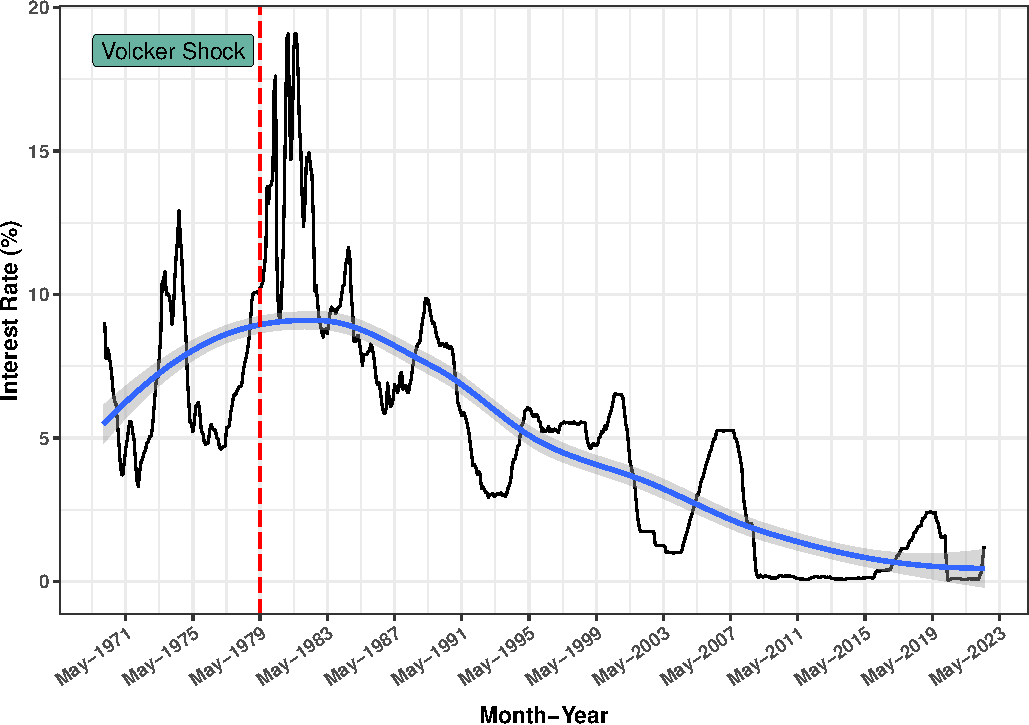
\includegraphics{fed-paper-drafting_files/figure-latex/fed_funds-1} 

}

\caption{\label{fed_funds_rate}Effective Federal Funds Rate (\%)}\label{fig:fed_funds}
\end{figure}

\begin{figure}[ht]

{\centering 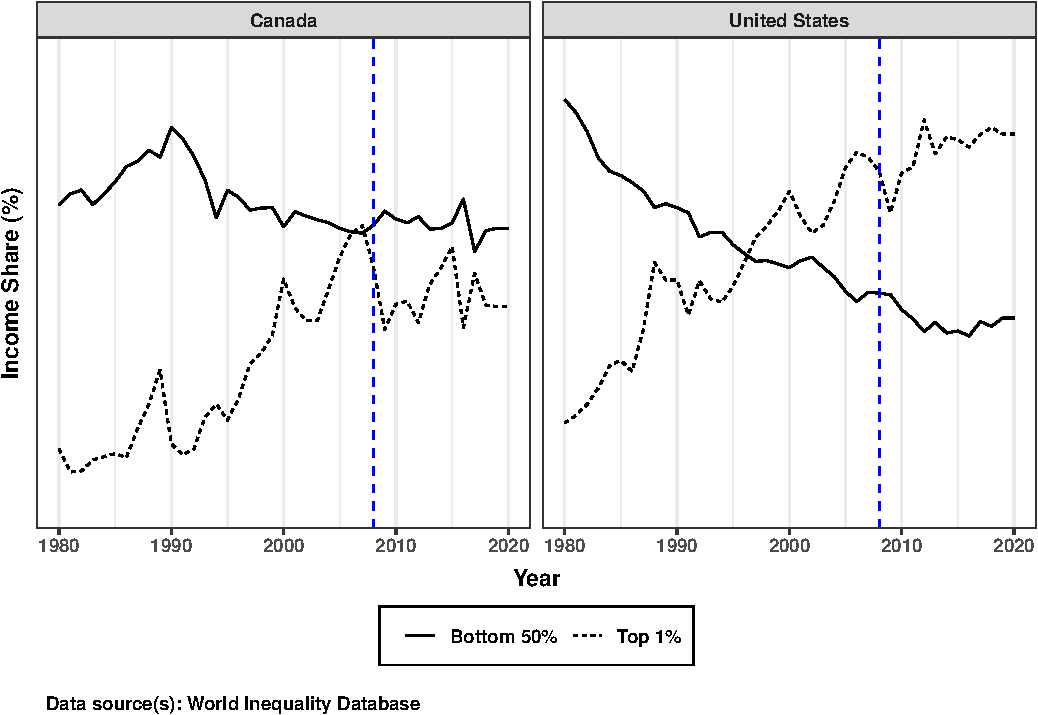
\includegraphics{fed-paper-drafting_files/figure-latex/income_dist1-1} 

}

\caption{\label{income_dist1}Share of National Income (\%)}\label{fig:income_dist1}
\end{figure}

\begin{figure}[ht]

{\centering 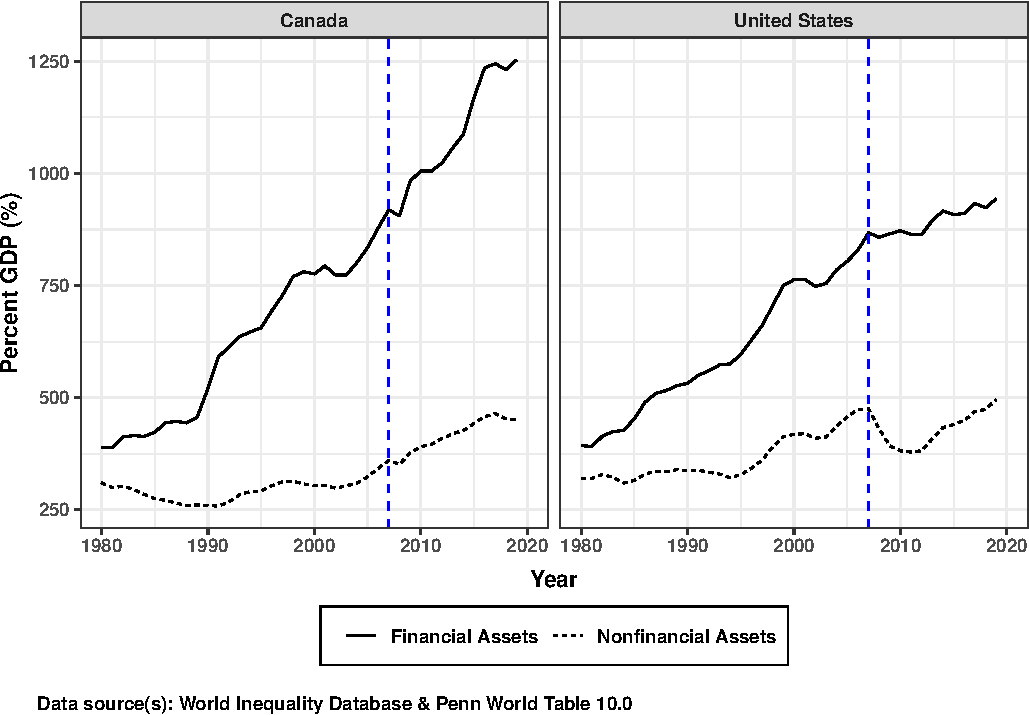
\includegraphics{fed-paper-drafting_files/figure-latex/capital_comp-1} 

}

\caption{\label{income_dist1}Cross-National Comparison of Capital Investments (\% of GDP)}\label{fig:capital_comp}
\end{figure}

\end{document}
